% Source of Bapmcm26202913_paper_zh_extended.pdf. Build in this folder with two runs of
%   xelatex -jobname=Bapmcm26202913_paper_zh_extended main.tex
% (fonts: TeX Gyre Termes/Heros, STIX Two Math, Noto Serif CJK SC) and copy Bapmcm26202913_paper_zh_extended.pdf to ../
\documentclass[a4paper,11pt]{article}
\usepackage{fontspec}
\setmainfont{TeX Gyre Termes}
\setsansfont{TeX Gyre Heros}
\newfontfamily\cjkfont{Noto Serif CJK SC}
\usepackage{amsmath}
\usepackage{unicode-math}
\setmathfont{STIXTwoMath-Regular.otf}
\usepackage[a4paper,top=2.5cm,bottom=2.4cm,left=2.6cm,right=2.6cm]{geometry}
\usepackage{graphicx,booktabs,array,threeparttable,pdfpages,fancyhdr,xurl}
\usepackage[font=small,labelsep=period,skip=4pt]{caption}
\usepackage[hidelinks,bookmarksnumbered=true,bookmarksopen=true]{hyperref}
\usepackage{titlesec}
\renewcommand{\floatpagefraction}{0.8}\renewcommand{\topfraction}{0.88}\renewcommand{\bottomfraction}{0.7}\renewcommand{\textfraction}{0.1}
\usepackage{etoolbox}\AtBeginEnvironment{thebibliography}{\small\linespread{1.05}\selectfont\setlength{\itemsep}{1pt}\setlength{\parskip}{0pt}}
\setlength{\emergencystretch}{3em}
\linespread{1.15}
\setlength{\parskip}{0.25em}
\titleformat{\section}{\large\bfseries}{E\arabic{section}}{0.8em}{}
\titleformat{\subsection}{\normalsize\bfseries}{E\arabic{section}.\arabic{subsection}}{0.6em}{}
\renewcommand{\thesection}{E\arabic{section}}
\renewcommand{\thefigure}{E\arabic{figure}}
\renewcommand{\thetable}{E\arabic{table}}
\renewcommand{\theequation}{E\arabic{equation}}
\setlength{\headheight}{15pt}\pagestyle{fancy}\fancyhf{}\renewcommand{\headrulewidth}{0.4pt}
\newcommand{\hd}[1]{\begin{tabular}[b]{@{}c@{}}#1\end{tabular}}
\newcommand{\exthead}[1]{\fancyhead[L]{\small #1}\fancyhead[R]{\small Part II\quad Post-competition extensions}\fancyfoot[C]{\small E-\thepage}}

\graphicspath{{../../figures/extension/}}
\hypersetup{pdftitle={Manifold micro-channel chip cooling -- extended edition}}
\begin{document}
\thispagestyle{empty}
\begin{center}
{\Large\bfseries Manifold Micro-Channel Chip Cooling: Surrogate Modelling,\\[0.2em] Multi-Objective Design and Tolerance Analysis}\\[0.7em]
{\large Extended edition --- note}
\end{center}
\vspace{0.8em}

This file has two parts. Part I is the paper submitted to Problem B of the 16th APMCM Asia-Pacific Mathematical Contest in Modeling (Chinese track), 2026 (43 pages, in Chinese), reproduced exactly as submitted. Part II, starting on page E-1, contains post-competition extensions written in November 2026.

The paper follows a chain of grey-box physics, dual surrogates, three-objective optimisation, preference robustness and tolerance sensitivity, and recommends the design $(0.22, 4.5, 4)$. Part II tests the surrogate layer itself and its effect on the conclusions. E1, a leave-one-level-out validation, finds that the thermal resistance in the attachment data is an exact cubic polynomial, and that the GPR intervals which cover 92--100\,\% of points under leave-one-out cross-validation cover only 31--77\,\% of a held-out level; universal kriging with a cubic trend restores 81--98\,\%. E2 propagates the surrogate uncertainty to the decision: the recommended design is the ideal-point choice in 100\,\% of draws from the universal-kriging posterior. E3 locates the next batch of CFD runs by posterior variance reduction. E4 repeats the tolerance analysis of Problem 5 on 1\,000 posterior surfaces; it confirms the tolerance conclusion but shows that the paper's GPR understates the tolerance spread of the thermal resistance and of the temperature non-uniformity by 16--28\,\%.

Every number in Part II can be reproduced with the scripts in the \texttt{extension/} folder of the code repository; result files are in \texttt{results/extension/}.

\clearpage
\pdfbookmark[0]{Part I\quad Competition paper (as submitted)}{part1}
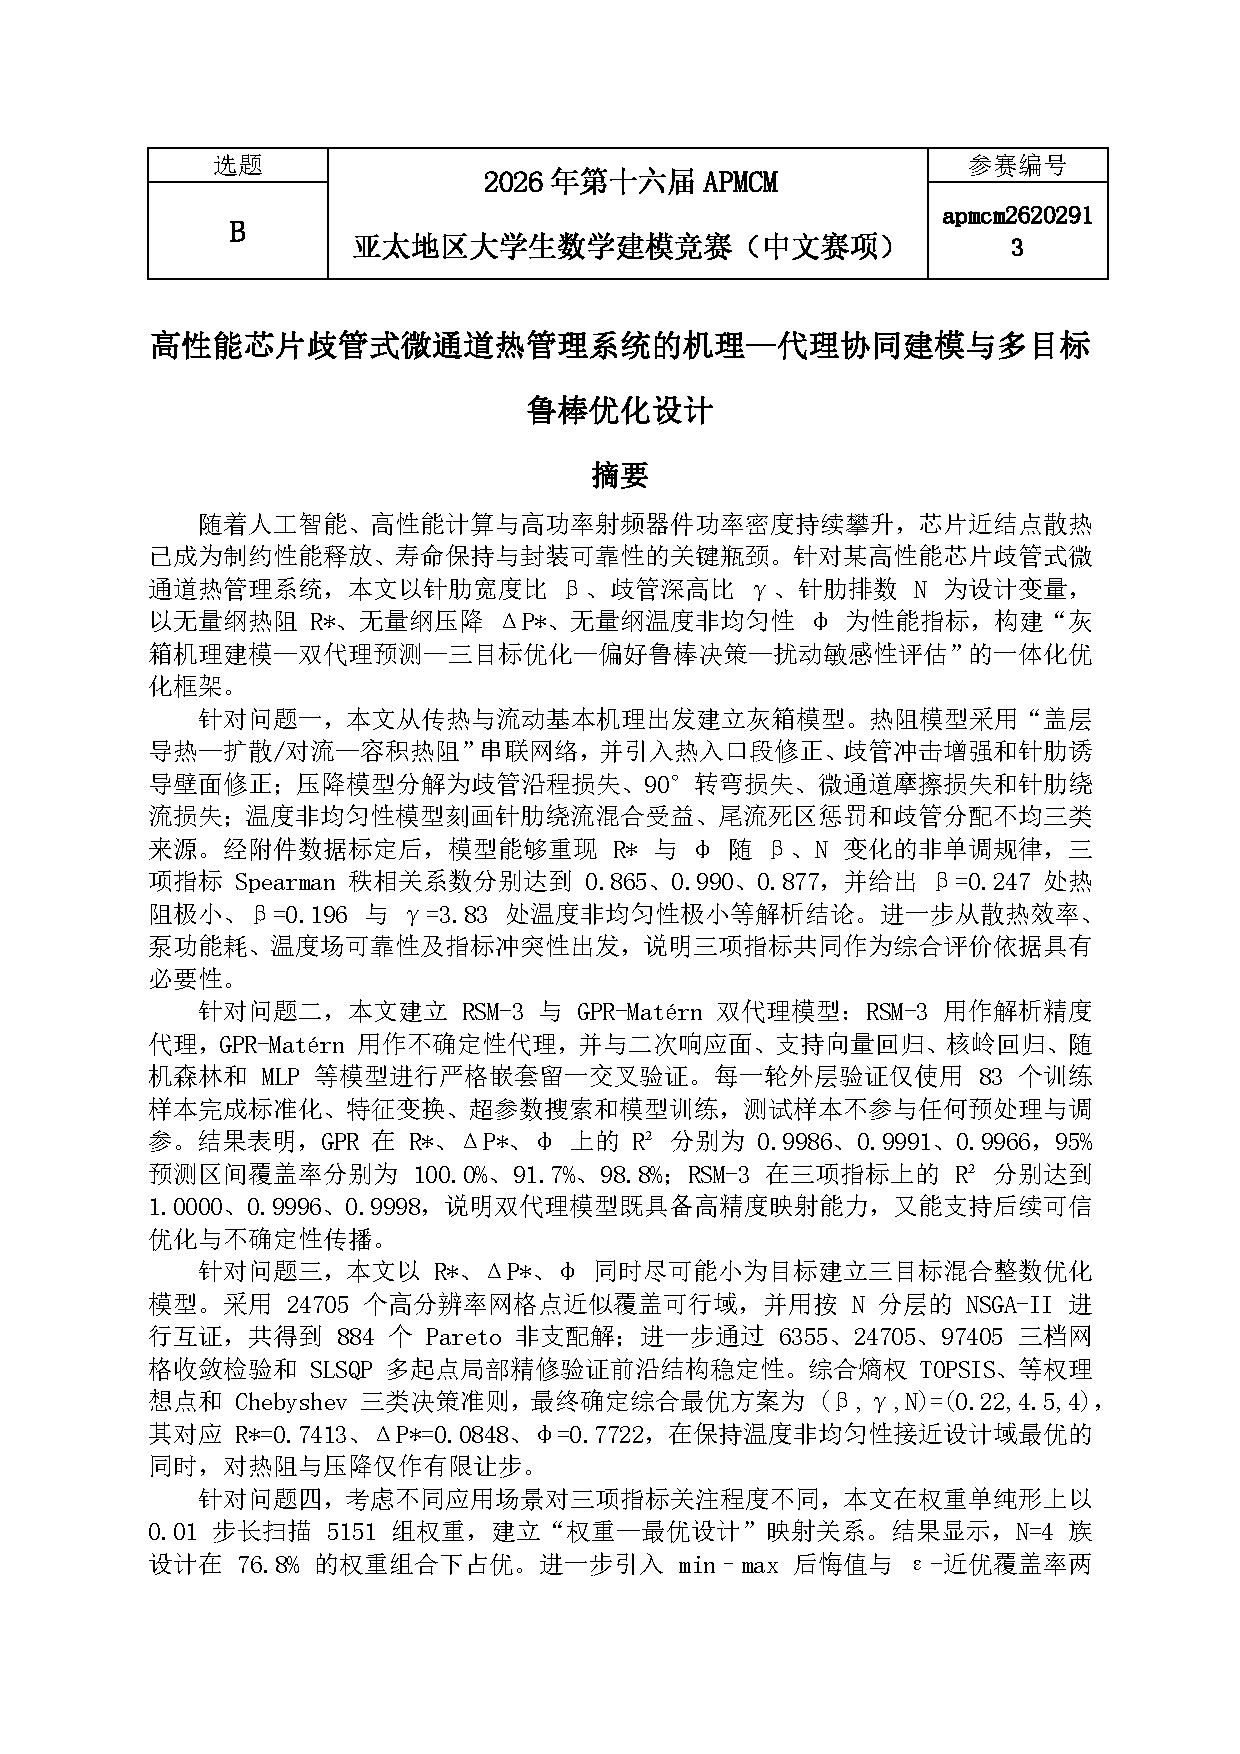
\includepdf[pages=-]{../Bapmcm26202913_paper_zh.pdf}
\pdfbookmark[0]{Part II\quad Post-competition extensions}{part2}
\setcounter{page}{1}
\exthead{Manifold micro-channel chip cooling}
\begin{center}{\Large\bfseries Part II\quad Post-competition extensions}\end{center}

The paper fits surrogate models of three responses, the thermal resistance $R^*$, the pressure drop $\Delta P^*$ and the temperature non-uniformity $\phi$, to the 84 CFD samples of the attachment: a cubic response surface (RSM-3) and Gaussian-process regression (GPR). On this basis it carries out a three-objective optimisation, a preference-robustness analysis and a manufacturing-tolerance analysis, and recommends the design $(\beta,\gamma,N)=(0.22, 4.5, 4)$. Its uncertainty analysis covers preferences (Problem 4) and manufacturing and operating perturbations (Problem 5), but not the surrogate models themselves. The four extensions below examine, in turn, how well the surrogates extrapolate, how surrogate uncertainty affects the decision, where the next simulations should go, and how the tolerance analysis changes once surrogate uncertainty is included.

\section{Leave-one-level-out validation exposes what leave-one-out cannot}

On a grid design, leave-one-out cross-validation keeps every neighbour of the held-out point on the same grid line, so it measures interpolation within the grid. The recommended design sits on the upper boundary of $\gamma$ and inside the unsampled interval $0.20<\beta<0.30$, so the relevant question is whether the surrogates can predict an entirely unseen level. Each level of $\beta$, $\gamma$ and $N$ was therefore held out in turn (20 samples for a level of $\beta$ or $\gamma$, 16 for a level of $N$; the four pin-free base cases always stay in training), and RSM-3, the paper's GPR with a Matérn kernel and universal kriging with a cubic trend (UK)\cite{cressie1993} were refitted on the remaining samples. The two end levels of each variable are labelled boundary levels (extrapolation) and the others interior levels (interpolation).

\begin{table}[htbp]\centering\small\setlength{\tabcolsep}{5pt}
\caption{Leave-one-level-out validation: prediction error (RMSE in \% of the range of the full sample) and coverage of the 95\,\% prediction interval (mean over levels).}\label{tab:ch-e1}
\begin{tabular}{llcccc}\toprule
 & & \multicolumn{2}{c}{RMSE / range (\%)} & \multicolumn{2}{c}{95\,\% interval coverage}\\\cmidrule(lr){3-4}\cmidrule(lr){5-6}
Model & Response & Boundary levels & Interior levels & Boundary levels & Interior levels\\\midrule
GPR (paper) & $R^*$ & 14.58 & 3.24 & 0.41 & 0.63\\
 & $\Delta P^*$ & 4.76 & 1.19 & 0.48 & 0.77\\
 & $\phi$ & 19.93 & 4.61 & 0.31 & 0.45\\\midrule
RSM-3 & $R^*$ & 0.001 & 0.001 & --- & ---\\
 & $\Delta P^*$ & 0.71 & 0.34 & --- & ---\\
 & $\phi$ & 0.60 & 0.31 & --- & ---\\\midrule
UK (cubic trend) & $R^*$ & 0.001 & 0.001 & 0.89 & 0.81\\
 & $\Delta P^*$ & 0.71 & 0.36 & 0.66 & 0.84\\
 & $\phi$ & 0.60 & 0.31 & 0.98 & 0.96\\\bottomrule
\end{tabular}
\end{table}

The first finding is that $R^*$ in the data is an exact cubic polynomial. A full cubic in $(\beta,\gamma,N)$ reproduces all 84 values of $R^*$ with a largest residual of $5.2\times10^{-7}$, which is the six-decimal rounding of the data, and it predicts entire held-out levels with an error of the same order (0.001\,\% for RSM-3 and UK in Table~\ref{tab:ch-e1}). The $R^2=1.0000$ of RSM-3 is therefore an identification of the surface that generated the data, not evidence of surrogate skill; $\Delta P^*$ and $\phi$ carry genuine cubic residuals, with maxima of 2.6\,\% and 1.6\,\% of their ranges. The second finding is that GPR intervals do not transfer to unseen levels. The 95\,\% intervals that cover 92--100\,\% of the points under leave-one-out cross-validation cover on average only 31--77\,\% of a held-out level, and 41\,\% for $R^*$ and 31\,\% for $\phi$ on boundary levels. The defect appears exactly where the recommended design lies. When the level $\gamma=4.5$ is held out, the GPR intervals cover 5\,\% ($R^*$, $\phi$) and 30\,\% ($\Delta P^*$) of the held-out samples, against 70\,\%, 100\,\% and 100\,\% for UK; when $\beta=0.3$ is held out, GPR covers none of the samples for any of the three responses, and its RMSE for $\phi$ reaches 50.8\,\% of the range. Universal kriging with a cubic trend repairs most of the calibration (mean coverage 81--98\,\%, except 66\,\% for $\Delta P^*$ on boundary levels) while matching the accuracy of RSM-3 (Figure~\ref{fig:ch-e1}). This agrees with the structure of the two models: the cubic trend absorbs the global shape of the response, so the Gaussian process only has to describe small residuals, whereas a pure Matérn model reverts to a constant mean away from the data and therefore extrapolates with both bias and overconfidence.

\begin{figure}[htbp]\centering
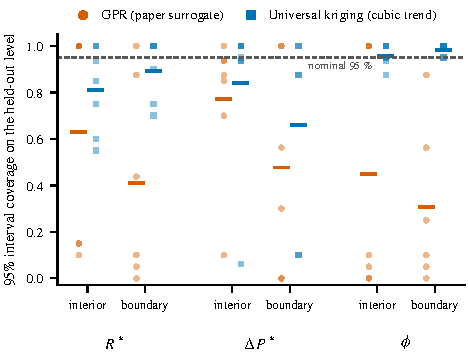
\includegraphics[width=0.7\textwidth]{figE1_level_holdout_coverage.pdf}
\caption{Coverage of the 95\,\% prediction intervals under leave-one-level-out validation: GPR against universal kriging with a cubic trend (UK).}\label{fig:ch-e1}
\end{figure}

\section{Is the recommendation robust to the surrogate itself?}

The remaining source of uncertainty is the surrogate fitted to 84 samples. E2 draws 1\,000 joint posterior samples of the three response surfaces on a design grid of 3\,255 points, extracts the Pareto front of each draw and applies the paper's three compromise rules. Under the calibrated universal-kriging posterior, $(0.22, 4.5, 4)$ is non-dominated in 100\,\% of the draws and is the choice of the equal-weight ideal-point rule in 100\,\% of the draws. Under the paper's GPR posterior the point itself wins in 82.9\,\% of the draws and its neighbourhood of $\pm1$ grid step in 100\,\%. The decision rule matters more than the surrogate: entropy-weighted TOPSIS always selects $N=2$ (91.6\,\% of the draws choose $(0.22, 4.5, 2)$), and the Chebyshev rule selects $N=6$. The paper's choice of the ideal-point rule, not surrogate error, is therefore the decisive modelling step.

\section{Where should the next CFD runs go?}

Because the posterior variance of a Gaussian process does not depend on outputs not yet observed, a batch of five new simulations was chosen greedily to minimise the posterior variance over the decision-relevant region, that is, over designs with uncertain Pareto membership or a non-zero probability of winning. Both surrogates point to the same gap: four of the five proposed runs lie at $\beta\approx0.24$--$0.25$ and $\gamma\approx3.2$--$3.55$, inside the unsampled interval of $\beta$, and the five runs would remove 21\,\% (universal kriging) to 53\,\% (GPR) of the posterior variance in the decision region (Figure~\ref{fig:ch-e3}).

\begin{figure}[htbp]\centering
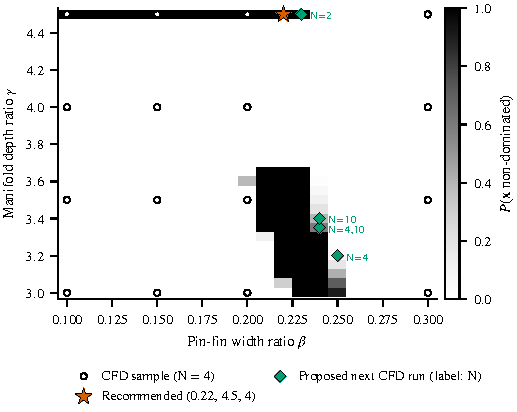
\includegraphics[width=0.66\textwidth]{figE2_posterior_pareto_N4.pdf}
\caption{Posterior probability that a design belongs to the Pareto front, on the slice $N=4$.}\label{fig:ch-e3}
\end{figure}

\section{The tolerance analysis of Problem 5 with the surrogate's own uncertainty}

\subsection{Design}
Problem 5 propagates manufacturing tolerances through the GPR surrogate and treats the surrogate as the truth: the standard deviation is 2\,\% of $\beta$ and 1.5\,\% of $\gamma$, with truncated normal distributions inside the design box. E4 repeats the analysis on 1\,000 joint posterior draws of the calibrated universal-kriging surfaces. Each draw is evaluated exactly at 4\,001 Monte Carlo inputs, namely the tolerance sample, its Sobol column swaps and the nominal design; first-order Sobol indices use the centred Jansen estimator\cite{jansen1999,saltelli2010}.

\subsection{Results}
\begin{table}[htbp]\centering\small\setlength{\tabcolsep}{5pt}
\caption{Tolerance-induced coefficient of variation (CV) and surrogate uncertainty at the recommended design $(0.22, 4.5, 4)$, all in \% of the nominal value.}\label{tab:ch-e4}
\begin{threeparttable}
\begin{tabular}{lcccc}\toprule
 & \multicolumn{2}{c}{Tolerance-induced CV} & Worst shift & Surrogate s.d.\\\cmidrule(lr){2-3}
Response & Paper (GPR) & UK posterior median [95\,\% band] & paper $\to$ UK & of nominal value\\\midrule
$R^*$ & 0.091 & 0.109 [0.109, 0.109] & 0.50 $\to$ 0.54 & $\approx 0$\tnote{a}\\
$\Delta P^*$ & 1.014 & 1.011 [0.968, 1.061] & 6.24 $\to$ 5.97 & 0.22\\
$\phi$ & 0.090 & 0.125 [0.120, 0.131] & 0.50 $\to$ 0.59 & 0.03\\\bottomrule
\end{tabular}
\begin{tablenotes}\footnotesize
\item[a] The universal-kriging surface of $R^*$ is the exact cubic polynomial that generated the data; its posterior standard deviation is about $10^{-5}\,\%$ of the nominal value.
\end{tablenotes}
\end{threeparttable}
\end{table}

\begin{figure}[htbp]\centering
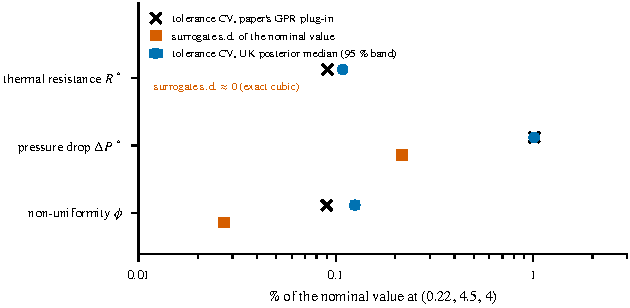
\includegraphics[width=0.84\textwidth]{figE3_tolerance_vs_surrogate.pdf}
\caption{Tolerance-induced coefficient of variation (the paper's GPR plug-in value; UK posterior median with the 95\,\% band over 1\,000 draws) and the posterior standard deviation of the nominal performance, all in \% of the nominal value.}\label{fig:ch-e4}
\end{figure}

The conclusion of Problem 5 survives the surrogate uncertainty (Table~\ref{tab:ch-e4}, Figure~\ref{fig:ch-e4}). The tolerance-induced coefficient of variation stays at or below about 1\,\% and is driven by $\gamma$: the first-order Sobol index of $\gamma$ exceeds that of $\beta$ in every posterior draw (posterior medians about 1.0 for $R^*$, 0.96 for $\phi$ and 0.76 for $\Delta P^*$). The paper's GPR, however, understates the tolerance spread of $R^*$ and $\phi$: its coefficients of variation are 16\,\% and 28\,\% below the universal-kriging values. For $R^*$ the universal-kriging surface is the exact cubic that generated the data (E1), so 0.109\,\% is the correct value under the stated tolerances; for the pressure drop the two agree. At the recommended design the remaining uncertainty is dominated by the tolerances rather than by the surrogate: for $\Delta P^*$ and $\phi$ the posterior standard deviation of the nominal performance is about one fifth of the tolerance-induced standard deviation (ratio 0.21--0.22), and for $R^*$ it is essentially zero (ratio about $10^{-4}$).

\subsection{Conclusions and limits}
Taken together, the four extensions show that the recommended design and its robustness conclusions withstand surrogate uncertainty, and that two things need improvement: the interval calibration of the GPR when it extrapolates to unsampled levels, and the data coverage of the unsampled interval $\beta\approx0.24$--$0.25$. All analyses take the 84 CFD samples of the attachment as the source of truth and add no new CFD simulations; the batch proposed in E3 needs actual simulations to confirm its variance reduction.

\begin{thebibliography}{9}
\bibitem{cressie1993} N. Cressie. \emph{Statistics for Spatial Data} (revised edition). Wiley, 1993.
\bibitem{jansen1999} M. J. W. Jansen. Analysis of variance designs for model output. \emph{Computer Physics Communications}, 117(1--2): 35--43, 1999.
\bibitem{saltelli2010} A. Saltelli, P. Annoni, I. Azzini, F. Campolongo, M. Ratto, S. Tarantola. Variance based sensitivity analysis of model output. Design and estimator for the total sensitivity index. \emph{Computer Physics Communications}, 181(2): 259--270, 2010.
\end{thebibliography}
\end{document}
